\documentclass[a4paper, 12pt, twoside]{article}
\def\magyarOptions{hyphenation=huhyphn}
\usepackage[hungarian]{babel}
\usepackage{ae,aecompl}
\usepackage[T1]{fontenc}
\usepackage[utf8]{inputenc}
\usepackage{textcomp}
\usepackage{anysize}
% left right up down
\marginsize{3.2cm}{2.8cm}{2cm}{2cm}
\usepackage{setspace}
\setstretch{1.2}
\frenchspacing
\usepackage{chemfig}
\usepackage{gensymb}
\usepackage{fancyhdr}
\usepackage{enumerate}
\usepackage{amsmath}
\usepackage{upgreek}
\usepackage{indentfirst}
\usepackage{sidecap}
\numberwithin{equation}{section}
\numberwithin{figure}{section}
\numberwithin{table}{section}
\usepackage{multicol}
\usepackage{float}
\setcounter{tocdepth}{1}
\pagestyle{empty}
% uncomment for hyperlinks
\usepackage{xcolor}
\usepackage[colorlinks = true,
            linkcolor = red,
            urlcolor  = blue,
            citecolor = blue,
            anchorcolor = blue]{hyperref}



\title{Fizikai Kémia Laboratóriumi Gyakorlatok}
\author{Kovács Barna \\ Kunsági-Máté Sándor\\ Kiss András\\ Géza Nagy \\ Katalin Ősz \\ Gábor Lente\\ \\ \\ \\ \\ \\

\includegraphics[width=0.2\textwidth]{fig/pte_logo.eps} \\
Általános és Fizikai Kémia Tanszék \\ Pécsi Tudományegyetem}

\begin{document}

\clearpage\maketitle
\thispagestyle{empty}
\newpage 
\tableofcontents
\newpage

\pagestyle{plain}
\fancyhead[LE,RO]{GYÓGYSZERBOMLÁS -- ,,GYB''}
\fancyhead[LO,RE]{\thesection}
\fancyfoot[LE,RO]{\thepage}
\fancyfoot[RE,LO]{\emph{Fizikai Kémia gyakorlatok gyógyszerész hallgatóknak}}

\setcounter{section}{7}
\section{Gyógyszerbomlás sebességének hőmérsékletfüggése}
\subsection{Bevezetés}

A gyakorlat során az \emph{Aspirin} (acetilszalicilsav) hidrolízisének kinetikailag elsőrendű reakciójának hőmérsékletfüggését vizsgáljuk.
A sebességi állandója a következőképpen adható meg:

\begin{equation}
\label{eq:divider}
        k
        =
        \frac
                {1}
                {t}
	\ln
	\frac{z}{z-x}
\end{equation}

ahol $t$ az idő, $z$ a reagens (jelen esetben a \emph{Aspirin}) kezdeti koncentrációja, $x$ pedig az elbomlott reagens koncentrációja.

A reakció sebessége vagy a sebességi állandó értéke függ a hőmérséklettől.
A hőmérsékletfüggést az \emph{Arrhenius egyenlet} írja le:

\begin{equation}
\label{eq:divider}
        \frac
                {d\ln k}
                {dT}
	=
	\frac
		{E}
		{\mathrm{R}T^2}
\end{equation}

melynek integrált alakja:

\begin{equation}
\label{eq:divider}
        k
        =
	A
	e^{-E/( \mathrm{R} T)}
\end{equation}

illetve

\begin{equation}
\label{eq:divider}
        \lg k
        =
        \lg A
	-\frac{E}{2.303 \mathrm{R}T}
\end{equation}

Az egyenletben $A$ a preexponenciális tényező, $E$ az aktiválási energia, és R a gázállandó (R$ = 8.314$ J/Kmol).
Az aktiválási energia meghatározható grafikus úton, ha az $\lg k - 1/T$ függvény meredekségét megmérjük és azt szorozzuk 2.303 $\times$ 8.314-el, amikor az $E$-t J/molban kapjuk meg.
Ha két hőmérsékleten megmérjük a reakciósebességi együtthatót ($k_1$-t és $k_2$-t $T_1$ és $T_2$ hőmérsékleten) az aktiválási energia a következő képlettel számítható ki:

\begin{equation}
	E
	=
	2.303
	\times
	8.314
	\lg
	\frac{k_1}{k_2}
	\frac{T_1 T_2}{T_1-T_2}
\end{equation}

\subsection{A gyakorlat kivitelezése}
Az \emph{Aspirin} hidrolízise kinetikailag elsőrendű folyamat és az alábbiak szerint játszódik le (\ref{fig:salicilsav}. ábra).

\begin{figure}
\centering
\schemedebug{false}
\schemestart
	\footnotesize \chemname{\chemfig{*6(-=-(-O-[::-60]([::-60]=O)-)=(-(-[::-60]OH)=[::60]O)-=)}}{Acetilszalicilsav}
	\footnotesize \+
	\footnotesize \chemfig{OH^{-}}\arrow(.mid east--.mid west){->[k][]}
	\footnotesize \chemname{\chemfig{*6(-=-(-OH)=(-([::-60]-OH)=[::60]O)-=)}}{Szalicilsav} + CH$_3$COO$^-$
\schemestop
\caption{Az acetilszalicilsav lúgos hidrolízise.}
\label{fig:salicilsav}
\end{figure}

A reakció szobahőmérsékleten igen lassú, ezért a méréseket magasabb hőmérsékleten végezzük.
A reakció sebességi együtthatójának meghatározásához ismerni kell a reaktáns vagy a termék koncentrációjának változását a reakcióidővel.
Jelen reakcióban a képződő szalicilsav Fe$^{3+}$ ionokkal alkotott stabil ibolyaszínű komplexét határozzuk meg spektrofotometriás módszerrel.
A lúgos közegben lejátszódó reakcióelegyből meghatározott reakcióidőnél ismert mennyiségű mintákat veszünk, a reakciót befagyasztjuk a hőmérséklet és a [OH$^-$] hirtelen csökkentésével.
Az előírt hígításokat követően a szalicilsav Fe(III)-komplexének koncentrációját spektrofotometriás úton meghatározzuk. Higításra lehet szükség, ha az abszorbancia 2 feletti, ekkor ugyanis a legtöbb műszer által mért érték nincs egyszerű egyenes arányosságban a koncentrációval, ami megbízhatatlan értéket eredményez. Célszerű ilyenkor $5 - 10 \times$ higítást végezni, és újramérni az abszorbanciát, majd megszorozni a higítással a koncentrációra kapott értéket.
A $t = \infty$ reakcióidőhöz tartozó termékkoncentrációkat, amelyek megfelelnek az \emph{Aspirin} kezdeti koncentrációjának, igen nagy reakcióidőnél vett mintából lehet meghatározni.
A méréseket két hőmérsékleten kell végrehajtani, ezeket a gyakorlatvezető határozza meg a gyakorlat kezdetén.
A reakció Arrhenius paramétereinek meghatározása érdekében ajánlott hőmérséklet 313 és 353 K.

1 db \emph{Aspirin} tablettát dörzsmozsárban elporítunk, és főzőpohárban kevés desztillált vízben oldunk, majd 100 cm$^3$-es mérőlombikokba szűrjük és jelig töltjük (törzsoldat). Az így kapott oldat telített lesz\footnote{Az \emph{Aszpirin} oldhatósága vízben $\sim$ 2 - 4 g / L, hőmérséklettől függően. Egy tabletta hatóanyagtartalma 500 mg.}.

\textbf{A reakció indítása és nyomon követése:}

\begin{enumerate}[(a)]
\item Az Aspirin kezdeti koncentrációjának ($z$) meghatározása. A törzsoldatból 2-2 cm$^3$ mintát csiszolatos dugós Erlenmeyer lombikokba (alacsony és magas hőmérséklet) pipettázunk, hozzáadunk 3-3 cm$^3$ 0.25 M NaOH oldatot és a lombikokat belehelyezzük a választott hőmérsékletű termosztátokba. A 60. percben a reakciót mindkét lombikban befagyasztjuk (a lombikokat jeges vízbe állítjuk, 2-2 cm$^3$ 0.25 M sósavoldatot és 3-3 cm$^3$ FeCl$_3$ oldatot pipettázunk beléjük, majd desztillált vízzel 100 cm$^3$-re hígítjuk őket.)

\item A $t$ időpillanatig elbomlott \emph{Aspirin} ($x$) koncentrációjának meghatározása. A törzsoldat maradékát a mérőlombikból két csiszolatos dugós Erlenmeyer lombikba töltjük át, kb. fele-fele térfogatban (nem mossuk!), termosztátba helyezzük őket, hozzápipettázunk 5 cm$^3$ pufferoldatot, és elindítjuk a stoppert ($t$ = 0). A lombik kivétele nélkül a bomlás 15, 20, 25, 30 és 35. percében 2 cm$^3$-es mintákat veszünk mindkét lombikból, amelyet az előkészített 25 cm$^3$-es mérőlombikokba töltünk. A lombikokat úgy készítjük elő, hogy belemérünk 0.5 cm$^3$ 0.25 M sósavoldatot, 0.5 cm$^3$ 0.1 M FeCl$_3$-at. Így a minta vételekor a lúgos hidrolízis leáll. Ne felejtsük el előzetesen feliratozni a lombikokat! A minta hozzáadását követően 25 cm$^3$ össztérfogatra hígítjuk őket desztillált vízzel. Érdemes egymáshoz képest $1 - 2$ perc eltolással indítani a két hőmérsékleten vizsgált bomlási reakciót, hogy ne kelljen egyszerre mintát venni a két lombikból.
\end{enumerate}

\textbf{Fényabszorpció mérése és koncentráció számolása}. Mind a kezdeti, mind a $t$ időpillanatban lévő koncentráció meghatározása spektrofotometriásan történik. A spektrofotométer kezelési leírása a készülék mellett megtalálható. A 2-es abszorbanciaérték felett a mintát higítani, és a számítások során a kapott eredményt korrigálni kell. (Pl. ha higítás után a számolt koncentráció 0.1 M, és a higítás $2\times$ volt, akkor az eredeti koncentráció 0.2 M.) A minta \emph{Aszpirin}-koncentrációját úgy számítjuk ki, hogy a kapott abszorbaciaértéket megszorozzuk $b = 8.3~(mol/dm^3) / AU$ arányossági tényezővel. Ez annak a hipotetikus \emph{Aszpirin}-oldatnak a koncentrációja, melynek abszorbanciája egységnyi, ha $d = 1~cm$, ahol $d$ a rétegvastagság.


\subsection{Beadandó eredmények}

\begin{enumerate}
\item A mérési és számított adatok táblázatosan (\ref{table:tablazatos}. táblázat).
\item A sebességi állandók számítása (\ref{table:seb}. táblázat)\footnote{Standard deviáció, $s=\sqrt{\frac{\Sigma(x_i-\overline{x})^2}{n-1}}$}.
\item A sebességi állandó hőmérsékletfüggéséből határozzuk meg a sebességi állandó értékét 20 $\celsius$-on (293 K) grafikusan, ábrázolva a $\lg k$-t az $1/T$ függvényében.
\item Az Arrhenius egyenlet integrált alakjába történő behelyettesítéssel számítsuk ki az $E$ aktiválási energiát és a preexponciális tényezőt:
	\begin{enumerate}
		\item E [kJ mol$^{-1}$]
		\item $\lg$ A [$s^{-1}$]
		\item A [s$^{-1}$]
	\end{enumerate}
\end{enumerate}

\begin{table}[!h]
\caption{A mérési és számított adatok táblázatosan.}
\centering
T = ... K, $z$ = ... mg/100 cm$^3$
\begin{tabular}{|c|c|c|c|c|c|}
\hline
Reakcióidő, s&Hígítás&A&x, mg / 100 cm$^3$ &(z-x), mg / 100 cm$^3$ & $k$, s$^{-1}$ \\
\hline
... & ... & ... & ... & ... & ... \\
\end{tabular}
\label{table:tablazatos}
\end{table}

\begin{table}[!h]
\caption{A sebességi állandó hőmérsékletfüggése.}
\centering
\begin{tabular}{|c|c|c|c|c|}
\hline
Hőmérséklet, K& 1/T & $\overline{k}$ (átlag), s$^{-1}$ & $\lg k$ & standard deviáció \\
\hline
... & ... & ... & ... & ... \\
\end{tabular}
\label{table:seb}
\end{table}

\newpage
\clearpage
\section{Szelektivitási együttható meghatározása}
\subsection{Bevezetés}

Az ionszelektív elektródok olyan potenciometriás érzékelők, melyek valamely ion aktivitásának többé-kevésbé szelektív meghatározását teszik lehetővé.
Az ionszelektív elektródokat kiterjedten alkalmazzák a klinikai gyakorlatban: az automata analizátorokban a vér ill. szérum pH-jának, Na$^+$-ion és K$^+$-ion aktivitásának meghatározására ionszelektív elektródok szolgálnak. Könnyen határozható meg ion-szelektív elektróddal például csapvíz F$^-$-ion koncentrációja Cl$^-$-ion zavaró ion jelenlétében is, európiummal dópolt lantán fluorid kristályt használva ionszelektív membránként.

Az ionszelektív elektródok potenciálját ideális esetben (zavaró ionok hiányában) a Nernst-egyenlettel adhatjuk meg:

\begin{equation}
\label{eq:nernst}
	E
	=
	E^0
	+\frac{RT}{z_i F}
	ln(a_i)
\end{equation}

ahol $z_i$ az elektród által érzékelt elsődleges ion előjellel vett töltése, $a_i$ az aktivitása.
Az egyenletnek megfelelően kationokra érzékeny elektród esetén növekvő elsődleges ionaktivitásnál az elektród potenciálja nő, míg anionokra érzékeny elektródok esetén csökken.
Az ionszelektív elektródok nem minden esetben tekinthetők szigorúan vett reverzibilis elektródoknak, ezért elektródpotenciáljuk megadására gyakran a következő összefüggést alkalmazzák:

\begin{equation}
\label{eq:exp}
	E
	=
	E^0
	\pm S ln(a_i)
\end{equation}

ahol $S$ az elektród meredekségét jelenti, melyet külön méréssel célszerű megállapítani.
Reális, több komponenst is tartalmazó mintaoldatok esetén az ionszelektív elektródok potenciálját nem csak az elsődleges ionok aktivitása befolyásolja, hanem többé-kevésbé az oldatban lévő minden más ion is.
Ezeket zavaró ionoknak szokás nevezni, mivel megváltoztatják az elektród potenciálját.
Emiatt az \ref{eq:nernst} ill. \ref{eq:exp} egyenlet alkalmazása az elsődleges ionok aktivitásának meghatározásakor hibát okoz.
A mintaoldatban jelenlévő egyéb ionoknak az elektród potenciáljára gyakorolt hatását az úgynevezett potenciometriás szelektivitási együtthatóval ($k_{pot}$) tudjuk figyelembe venni.
Ennek felhasználásával az elektród potenciálját a Nikolskij-egyenlet írja le:

\begin{equation}
\label{eq:nikolsky}
E=E^0 + \frac{RT}{z_iF} \ln \left [ a_i + \sum_{j} \left ( k_{ij}a_j^{z_i/z_j} \right ) \right ]
\end{equation}

ahol $a_j$ a $j$-edik zavaró ion aktivitása, $z_j$ a töltése, $k_{pot}$ $i, j$ a $j$-edik zavaró ionra vonatkozó szelektivitási együttható.
A szelektivitási együttható értéke azt mutatja meg, hogy az elektród az $i$ elsődleges iont hányszor érzékenyebben jelzi, mint a $j$ zavaró iont.
Például $k = 10^{-2}$ esetén a $j$ ion aktivitása százszor nagyobb kell, hogy legyen az elsődleges ion aktivitásánál ahhoz, hogy ugyanakkora mértékben vegyen részt a potenciál kialakításában, mint az $i$ ion, hogy ugyanakkora mértékben vegyen részt a potenciál kialakításában, mint az $i$ ion.

A szelektivitási együttható meghatározására két módszer terjedt el: az úgynevezett kevert oldatos és az ún. különoldatos módszer.

A kevert oldatos módszer esetén állandó $j$ zavaró ion aktivitás mellett változtatjuk az elsődleges $i$ ion aktivitását.
A mérési adatok ábrázolásával nyert diagramból \ref{fig:Q} meghatározzuk a $Q$ metszéspontot.
Ennek adataiból a szelektivitási koefficiens a

\begin{equation}
\label{eq:szel1}
	k_{i,j}^{pot}
	=
	\frac{(a_i^{z_j})_Q}{a_j^{z_i}}
\end{equation}

összefüggéssel számítható ki.

\begin{figure}
\centering
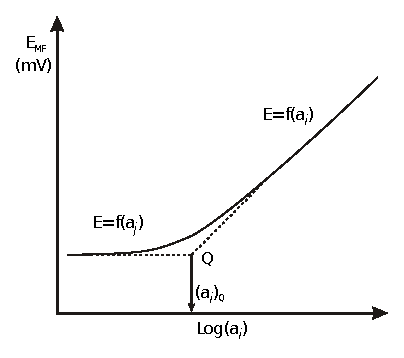
\includegraphics{fig/ion1.eps}
\caption{Ionszelektív elektród szelektivitási együtthatójának meghatározása kevert oldatos módszerrel kapott adatokból.}
\label{fig:Q}
\end{figure}

A külön oldatos eljárás alkalmazásakor két görbe felvételére van szükség.
Zérus zavaró ion aktivitás mellett fel kell venni az elsődleges $i$ ionra vonatkozó kalibrációs görbét, majd egy másik mérés során zérus elsődleges ion aktivitás mellett meg kell határozni a $j$ zavaró ionra vonatkozó kalibrációs görbét.
Amint a 2. ábra mutatja, a két görbe segítségével a szelektivitási együttható értéke meghatározható az

\begin{enumerate}[(a)]
\item azonos poteniálokhoz tartozó aktivitások arányából

\begin{equation}
\label{eq:azonospot}
        k_{i,j}^{pot}
        =
        \frac{a_i}{a_j^{z_i/z_j}}
\end{equation}

\item az azonos aktivitásokhoz tartozó potenciálokból:

\begin{equation}
\label{eq:azonosakt}
        \lg k_{i,j}^{pot}
        =
        \frac{(E_2-E_1)zF}{2.303RT}
	=
	\frac{\Delta E}{S}
\end{equation}

\end{enumerate}

A szelektivitási együttható értékét számos tényező befolyásolja: a mintaoldat ionerőssége, a meghatározás módja, stb.
Látható az \ref{eq:azonospot}. és \ref{eq:azonosakt}. összefüggésekből a külön oldatos módszer hátránya: feltételezi, hogy az elsődleges és zavaró ionok töltése megegyezik, továbbá hogy az elektród meredeksége mindkét ionra azonos.
A külön oldatos módszernél a meghatározás körülményei a gyakorlatban felmerülő analízis körülményeitől eltérhetnek, ezért az így meghatározott szelektivitási együttható értékek közelítő értékeknek tekinthetők.

\begin{figure}
\centering
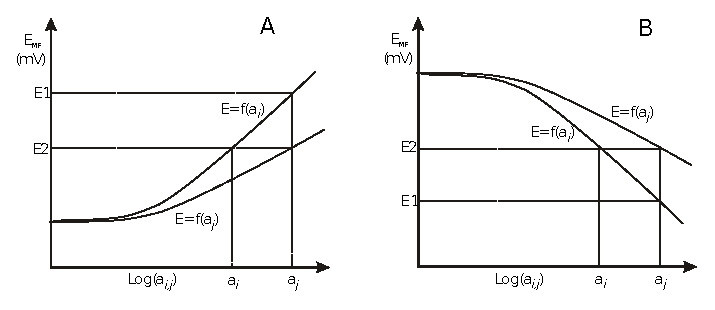
\includegraphics{fig/ion2.eps}
\caption{A szelektivitási együtthatók meghatározása külön oldatos módszerrel. (A) Egyszeresen pozitív, és (B) egyszeresen negatív töltésű ionokra.}
\label{fig:ion2}
\end{figure}

\subsection{A gyakorlat leírása}
A gyakorlat célja a kálium-ion vagy fluorid-ion (kérdezze a gyakorlatvezetőtől) szelektív elektród funkcióinak vizsgálata.
Első feladatként meg kell határozni, hogy az elektród milyen aktivitástól képes – a Nernst egyenletnek megfelelően – az elsődleges ion aktivitásának mérésére.
Ehhez hígítási sort készítünk a megfelelő elsődleges ion sójából (KCl ill. NaF).
100 ml mérőlombikban készítsen 10$^{-2}$ mol$\cdot$dm$^{-3}$ koncentrációjú oldatot az elsődleges ion sójából.
10-szeres hígításhoz 10 ml-t pipettázzon át egy másik 100 ml mérőlombikba, és töltse jelre ioncserélt vízzel.
A hígítást addig ismételje új mérőlombikban mindig az előző oldatot felhasználva, míg el nem éri a 10$^{-6}$ mol$\cdot$dm$^{-3}$ koncentrációt.
Az oldatokat öntsük ki feliratozott főzőpoharakba.
Az elektródot a leghígabb oldatot tartalmazó edénybe merítjük a vonatkoztatási elektróddal együtt és csatlakoztatjuk a pH mérő megfelelő bemeneteihez.
Kb. 1 perc elteltével olvassuk le és jegyezzük fel az elektródpotenciál értékeket.
Leolvasás után merítsük az elektródokat a következő, tízszer töményebb oldatba és ismét 1 perc elteltével olvassuk le az elektródpotenciál értéket.
A mérést végezzük el mind az öt oldatban, a leghígabbtól a legtöményebb felé haladva háromszor egymás után.
A mérési sorozatok között és után alaposan öblítsük le az elektródot és a mérőedényt mossuk ki ioncserélt vízzel.

\subsubsection{A szelektivitási együttható meghatározása kevert oldatos eljárással}

A továbbiakban ismételjük meg a mérést, azonban a hígítási sor készítéséhez ioncserélt víz helyett 10$^{-2}$ mol$\cdot$dm$^{-3}$ koncentrációjú NaCl, oldatot használjunk (zavaró ion Na$^+$, illetve Cl$^-$ a K$^+$, illetve F$^-$ ion-szelektív elektród esetére).
Mivel a mérésekkor termosztálást nem alkalmaztunk, jegyezzük fel a laboratórium hőmérsékletét.
Fontos, hogy az oldatok készítéséhez kálium, nátrium, klorid és fluorid ionoktól mentes vizet használjunk.

\subsubsection{A szelektivitási együttható különoldatos eljárással}

Az elektródok leöblítése után határozzuk meg az elektród szelektivitási együtthatóját külön oldatos módszerrel.
Ehhez a zavaró ion sójából készítünk hígítási sort, a 2. pont bevezetésében leírt módszerrel.
Mivel a zavaró ionra az ion-szelektív elektród (ideálisan) sokkal kevésbé érzékeny, ezért nagyobb koncentrációt kell alkalmaznunk, hogy vizsgálhassuk a zavaró hatást.
A mérés befejeztével öblítsük le az elektródot és a mérőedényt mossuk ki ioncserélt vízzel.

\subsection{A gyakorlat kiértékelése}

A koncentrációk, aktivitási koefficiensek és a térfogat értékek ismeretében számítsa ki az oldatok elsődleges ion aktivitását.
Ábrázolja a mért potenciálértékeket az elsődleges ion aktivitás logaritmusának függvényében.

A kevert oldatos mérések során felvett, a különböző oldatokban nyert görbéket ábrázolja egy diagramban.
Határozza meg minden mérési sorozatból az elektród meredekségét.
A csak elsődleges ionok jelenlétében felvett görbéből határozza meg a grafikusan az elektród kimutatási határát is.

A kevert oldatos mérésekből az 1. ábrán bemutatott módon határozza meg a (4) egyenlet alkalmazásával a szelektivitási együttható értékeit a különböző klorid ion aktivitások mellett.
Ábrázolja a szelektivitási együttható értékét a kloridion aktivitás függvényében.

A különoldatos módszerrel történő kiértékeléshez egy diagramban ábrázolja az elektród potenciált az illető ion aktivitásának függvényében (egyszer az elsődleges, egyszer a zavaró ion esetén).
Figyelembe kell vennie, hogy a közepes aktivitási koefficiensek eltérőek lehetnek.
A két görbéből a 2. ábrának megfelelően két, azonos aktivitáshoz tartozó potenciálnál, valamint azonos potenciálhoz tartozó két aktivitásból is számítsa ki a szelektivitási együttható értékét.

\subsection{Beadandó eredmények}
Az elektród kimutatási határa, 3 szelektivitási együttható kevert, és 2 szelektivitási együttható külön oldatos módszerrel meghatározva.
Az elektród meredeksége azelsődleges ill. a zavaró ionokat tartalmazó oldatban. 5 kalibrációs görbe.


\newpage
\clearpage
\section{Gyengesav disszociációs állandójának meghatározása vezetés mérésével}
\subsection{Bevezetés}
Az elektromos ellenállás anyagi tulajdonság.
Ohm törvénye értelmében egy anyagon átfolyó elektromos áram erősége ($I$) és az áramot létrehozó feszültség ($U$) között egyenes arányosság van:

\begin{equation}
\label{eq:ohm}
	U
	=
	I
	\cdot
	R
\end{equation}

ahol az $R$ arányossági tényezőt az illető anyag ellenállásának nevezzük, mértékegysége az ohm ($\ohm$).
Fajlagos ellenálláson az 1 m hosszú, 1 m$^2$ (a gyakorlatban 1 mm$^2$) keresztmetszetű vezetőn az 1 amper intenzitású áram létrehozásához szükséges feszültség és az áram hányadosát értjük.

Az elektrokémiában több szempontból előnyös, ha a fenti mértékegységek reciprokait használjuk: az ellenállás reciprokát vezetésnek (mértékegysége a Siemens, S = 1/$\ohm$), a fajlagos ellenállás reciprokát fajlagos vezetésnek nevezzük.

Elektrolitok oldatainak fajlagos vezetésén ($\kappa$) az 1 cm távolságban, párhuzamos, 1-1 cm$^2$ felületű elsőrendű (inert fém, pl. arany vagy gyakrabban platina) vezetőből készült elektródok között elhelyezkedő folyadékkocka vezetését értjük, mértékegysége S $\cdot$ cm$^{-1}$.
A fajlagos vezetés függ az elektrolit anyagi minőségétől, koncentrációjától, valamint a hőmérséklettől.
Moláris fajlagos vezetésen ($\Lambda _m$) a fajlagos vezetés és a koncentráció hányadosát értjük. Ez alapján

\begin{equation}
\label{eq:lambdam}
        \Lambda_m
        =
        \frac
		{\kappa 1000 }
		{c}
	=
	\kappa V
\end{equation}

ahol $c$ az oldat koncentrációja (mol$\cdot$dm$^{-3}$) és $V$ a hígítás.
%A vezetés szoros kapcsolatban van az ionok mozgékonyságával: ha ugyanis a mérő elektródra feszültséget kapcsolunk, az elektrolitban ionvándorlás indul meg.
%A vándorlás sebessége függ az elektromos térerő nagyságától, ezért a vándorlási sebességet 1 V/cm térerőre vonatkoztatjuk.
%Az 1 V/cm térerő hatására másodpercenként megtett utat az ion relatív mozgékonyságának ($u$) nevezzük.
Mivel egy biner elektrolitban mind az anionok, mind a kationok hozzájárulnak a vezetéshez, erős elektrolitok híg oldatainak fajlagos moláris vezetését az \emph{ionok független vándorlásának törvénye} írja le:

\begin{equation}
\label{eq:kohlrausch2}
	\Lambda _m^0
	=
	\lambda _a^0 \nu _a z_a + \lambda _k^0 \nu _k z_k
%	/1000
\end{equation}

ahol $z_a, z_k$: ionok töltésszáma; $\nu _a, \nu _k$: sztöchiometriai konstansok; $\lambda _a^0$ illetve $\lambda _k^0$ az anionok és a kationok végtelen hígításra vonatkozó moláris fajlagos vezetése.
Gyengeelektrolitok vezetése

\begin{equation}
\label{eq:lambdam}
        \lambda_c
        =
        \alpha
	\lambda_0
\end{equation}

formában adható meg, ahol $\alpha$ a disszociáció foka, $\lambda _0$ a végtelen hígítású oldat moláris fajlagos vezetése.
%Ha a gyengeelektrolit koncentrációja kicsi, az ionmozgékonyságok csak a hőmérséklettől függenek, a koncentrációtól nem.
Egy AH gyengesav disszociációs állandója ($K_d$) kiszámítható a koncentráció és a disszociáció fokának ismeretében

\begin{equation}
\label{eq:kd}
        K_d
        =
        \frac{\alpha^2 c}{1-\alpha}
\end{equation}

Érdemes megjegyezni azonban, hogy a disszociációs állandó adott hőmérsékleten függ - a Debye-Hückel elmélet alapján - a közeg permittivitásától is.
Ha a \ref{eq:lambdam} egyenlet $\alpha$-ra rendezett alakját behelyettesítjük ez utóbbi egyenletbe, a gyengeelektrolitok disszociációjára Ostwald által megállapított összefüggéshez jutunk (\emph{Ostwald féle hígítási törvény}):

\begin{equation}
\label{eq:ostwald}
        K_d
        =
        \frac{\lambda_c^2 c}{\lambda_0^2 - \lambda_0\lambda_c}
\end{equation}

A disszociációs állandó értékét tehát vezetésméréssel meghatározhatjuk. 
$\lambda_c$ közvetlenül mérhető, míg $\lambda_0$ értékét az alábbiak szerint határozhatjuk meg:
A \ref{eq:ostwald} egyenlet átrendezésével

\begin{equation}
\label{eq:ostwald2}
        \frac{1}{\lambda_c}
        =
	\lambda_c
	c
	\frac{1}{K_d \lambda_0^2}
	+\frac{1}{\lambda_0}
\end{equation}

kifejezést kapjuk.
Ha ábrázoljuk $1/\lambda_c$-t $\lambda_c c$, azaz $\kappa$ függvényében, egyenest kapunk, melynek tengelymetszete $1/\lambda_0$. $\lambda_c$ és $\lambda_0$ ismeretében pedig $K_d$ értéke már kiszámítható.
A mérések kivitelezésekor a következőket kell figyelembe vennünk:
\begin{enumerate}[(a)]
\item Az oldat mért vezetéséhez az oldott anyag mellett az oldószer is hozzájárul.
Híg oldatok esetén ezért külön méréssel meghatározzuk az oldószer vezetését ($G_{\text{oldószer}}$) és ezt az értéket levonjuk az oldat esetében mért vezetés értékéből.

\item Az újabban használatos elektródok geometriája és elrendezésük eltérnek a fajlagos vezetés definíció szerinti meghatározásánál leírtaktól, ezért a mérőelektródot kalibrálni kell.
Az eltérés a mérést nem befolyásolja, mivel az eltérés az úgynevezett cellaállandó - mint kalibrációs paraméter - segítségével figyelembe vehető.
A cellaállandó (jele $C$, egysége m$^{-1}$ vagy cm$^{-1}$) megmutatja egy ismert fajlagos vezetésű oldat ($\kappa_{ref}$) és az adott mérőcellával ezen oldaton mért vezetés ($G_{\text{mért}}$) közötti kapcsolatot:

\begin{equation}
\label{eq:c}
	C
	=
	\kappa_{\text{ref}}/G_{\text{mért}}
\end{equation}

\end{enumerate}

Ezek alapján az oldat hozzájárulását a vezetéshez a következőképpen kapjuk meg: $\kappa_{\text{korr}} = (G_{\text{oldat}} - G_{\text{oldószer}})C$,
ahol $\kappa_{\text{korr}}$ az oldatnak a cellaállandóval és az oldószer fajlagos vezetésével korrigált értéke, $C$ a cellaállandó (nem tévesztendő össze a koncentrációval, melyet $c$-vel jelölünk).
Ezek alapján a gyengesav oldat moláris vezetése:

\begin{equation}
\label{eq:c}
        \lambda
        =
        \kappa_{korr}
	V
\end{equation}

ahol V a hígítás.

\begin{figure}
\centering
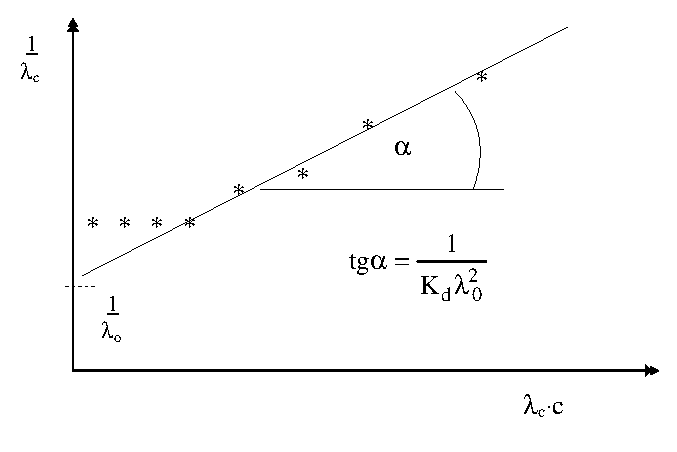
\includegraphics{fig/lambda0.eps}
\caption{Végtelen higítású oldat vezetésének ($\lambda_0$) meghatározása.}
\label{fig:}
\end{figure}

\subsection{A gyakorlat leírása}

A konduktométer harangelektródját többször (4 - 5) öblítsük át desztillált vízzel majd kis részlet 1 $\upmu$S/cm-nél kisebb fajlagos vezetésű vízzel, melyet külön edényben a technikustól kell kérni.
A gyakorlatvezető által kijelölt alkohollal (metanol, etanol vagy propanol) készítsünk 20 v/v\%-os oldatot.
A kijelölt 1 mol$\cdot$dm$^{-3}$ koncentrációjú gyengesav törzsoldatából pipettázzunk két száraz 100 cm$^3$-es mérőlombikba 2.00 cm$^3$-t, majd töltsük jelre az első lombikot vezetőképességi vízzel, a másikat a 20\%-os alkohol oldattal.
A mérést mérőhengerben végezzük.

Töltsük először a vizes hígítású oldatot a mérőedénybe, és mérjük meg a vezetését.
Ezután 25 cm$^3$-t pipettázzunk ki az oldatból és 50 cm$^3$-es mérőlombikban hígítsuk kétszeresére.
Az elektród gondos leöblítése után mérjük ezen oldat vezetését is.
%Az oldat vezetését leghelyesebb úgy meghatározni, hogy az elektród bemerítésétől 5 percen át 30-60 másodpercenként észleljük és feljegyezzük a cellában jelentkező vezetés értékeket.
A kétszeres hígítást még 3-4-szer megismételjük, minden alkalommal mérve a vezetést.

Ismételjük meg a méréseket az alkoholt tartalmazó oldatokkal is úgy, hogy a hígítások során bidesztillált víz helyett a mérőlombikot az alkoholos oldattal töltjük mindig jelre.

Minden esetben jegyezzük fel a mért oldat hőmérsékletét is (a vezetőképességmérő írja az elektródba épített hőmérő által mért hőmérsékletet).
%A mérőcellában egy-egy oldatot legalább 25 percig kell termosztálni.
%A rendelkezésre álló idő rövidsége miatt a legcélszerűbb, ha a sorozat következő, már meghígított tagját főzőpohárban előre a termosztátba helyezzük, így csökkentve a két mérés közti várakozási időt.

Végül mérjük meg mind a hígításokhoz használt vezetőképességi víz, mind az alkohol oldat vezetését, melyekkel mérési eredményeinket korrigálnunk kell.
Ezután határozzuk meg 0.1 és 0.01 M KCl oldatok felhasználásával a cellaállandó értékét úgy, hogy cellakonstansként a két mérésből számolt értékek átlagát fogadjuk el.

A \ref{fig:vez}. ábra egy vezetőképesség mérésére szolgáló cella felépítését mutatja.
A mérendő oldatba egy geometriailag jól definiált, indifferens elektródpárt merítünk és az ezen létrejövő feszültségesést mérjük.
A konduktometria gyakorlatban az elektrolízis, ill. az elektromos polarizáció csökkentése, ill. kiküszöbölése érdekében váltóárammal végezzük a mérést.

\begin{figure}
\centering
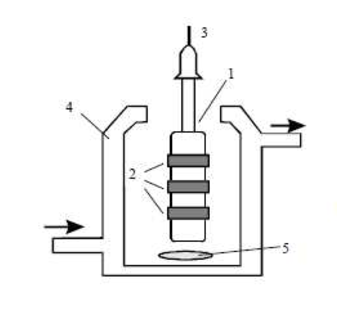
\includegraphics{fig/cond.eps}
\caption{Vezetőképesség mérésére szolgáló cella felépítése. 1 - harangelektród, 2 - Pt korommal bevont gyűrűk, 3 - elektromos elvezetés, 4 - kettős falú temperálható edény, 5 - mágneses keverő.}
\label{fig:vez}
\end{figure}



\subsection{A mérési eredmények kiértékelése}

\begin{enumerate}
\item Számítsuk ki a cellaállandó értékét.
A mérési eredményeket a vizes és az alkoholos sorozatnál is foglaljuk táblázatba:

\begin{table}[!h]
\centering
\begin{tabular}{|c|c|c|c|c|c|c|c|}
\hline
c (mol $\cdot$ dm$^{-3}$) & G$_{\text{mért}}$ & $\kappa_{\text{korr}}$ (S $\cdot$ cm$^{-1}$) & $\lambda_c$ & $1/\lambda_c$ & $\lambda_c c$ & $\alpha$ & $K_d$ \\
\hline
... & ... & ... & ... & ... & ... & ... & ... \\
\end{tabular}
\label{table:vez}
\end{table}

\item Határozzuk meg grafikusan $\lambda_0$ értékét, $\lambda_c$ és $\lambda_0$ ismeretében pedig minden koncentrációra számítsuk ki $\alpha$ és $K_d$ értékeit.

\end{enumerate}



\newpage
\clearpage
\section{Partition equilibrium of I$_2$ between two phases}
\subsection{Introduction}
If a two

Ha két, egymással nem elegyedő oldószerben egy anyag egyidejűleg oldódik, és a két oldószer érintkezésbe kerül egymással, az egyensúly beállása után az oldott anyagnak a két oldószerben érvényes aktivitásának (koncentrációjának) aránya állandó.
Egy ilyen, két fázisból (A és B) és három komponensből álló rendszernek a Gibbs-féle fázisszabály szerint három szabadsági foka van: a nyomás és hőmérséklet mellett a megoszló anyag koncentrációja az egyik fázisban.
A termodinamikai egyensúly adott hőmérsékleten és nyomáson - a megoszlást illetően - akkor áll be, mikor a megoszló anyag (x) kémiai potenciálja mindkét fázisban azonos lesz:
ux,A = ux,B
u*x,A + RT ln ax,A = u*x,B + RT ln ax,B
ahol u*x,i - a megoszló anyag standard kémiai potenciálja az i-edik fázisban
ax,i - az x-anyag aktivitása az i-edik fázisban
Az egyenletet átrendezve
(u*x,A - u*x,B) / R x T = ln ax,B / ln ax,A                (8.1)
látható, hogy az egyenlet bal oldala (adott hőmérsékleten és nyomáson) konstans.
Ezt megoszlási állandónak nevezzük.
(A logaritmus függvény monotonitása miatt az ax,B/ax,A hányadost is szokás használni, ezt megoszlási hányadosnak nevezzük.)
Az egyenlet értelmében a megoszlás nem függ a fázisokban mért abszolút koncentrációtól, csak ezek arányától.
Ez azonban csak egy fontos feltétel teljesülésekor igaz: nevezetesen abban az esetben, ha az oldott anyag egyik oldószerben sem szenved disszociációt, illetve nem alkot asszociátumokat sem.
Amennyiben e feltétel nem teljesül, a megoszlás igaz marad az oldott anyagra nézve, ha olyan analitikai technikával követjük koncentrációjának megváltozását, mely nem érzékeny az oldott anyagból valamely - vagy mindkét- oldószerben keletkező további - esetleg egyensúlyi- formákra.
Az elterjedt - és a gyakorlaton alkalmazott - mérési eljárások azonban olyanok, hogy csak az adott fázisban található összes oldott anyag meghatározására nyújtanak lehetőséget.
Így a fenti egyenlettől látszólagos eltérések tapasztalhatók.
Ezen eltérések azonban igen fontosak lehetnek számunkra: felvilágosítást adhatnak az oldott anyagnak az adott oldószerben kialakuló esetleges szerkezeti / disszociációs / asszociációs tulajdonságairól.
Tekintsünk egy egyszerű példát: a cA koncentrációjú A anyag a poláris fázisban legyen protonálható, így a poláris fázisbeli (v) összkoncentrációja cA,v = [A]v + [AH+]v.
Amennyiben az apoláris fázisba (o) csak az A forma extrahálható, a megoszlási állandóra nem a K = cA,o/cA,v, hanem a K = cA,0/[A]v kifejezést találjuk állandónak.
Ehhez hasonlóan a szerves fázisban is eltérő formában lehet jelen a megoszló komponens: pl. közismert, hogy organikus gyengesavak apoláris oldószerben gyakran dimereket, vagy magasabb rendű aggregátumokat képeznek.
Ilyen esetben szintén korrekciót kell alkalmaznunk, nevezetesen mindig meg kell keresnünk azt a komponenst, melyre a megoszlási egyensúly felírható, továbbá a lehetséges egyensúlyi formáinak figyelembevételével a tömeghatás törvény értelmében korrigálnunk kell az aktivitására/koncentrációjára vonatkozó összefüggéseket.

A fentiek alapján egy gyengesav vizes és szerves oldószeres fázisok között történő megoszlásakor mindkét hatással - tehát a vizes közegben bekövetkező disszociációval és a szerves fázisban történő asszociációval - is számolnunk kell.
Legyen cAH,v az AH gyengesav vizes közegben mért analitikai koncentrációja, és cAH,o a szerves fázisban mért összes koncentráció.
Minthogy vizes közegben a sav protonokra és savmaradékra disszociál, a vizes közegben lévő AH forma koncentrációja [AH] = cAH,v(1-alfa) alakban írható fel, ahol alfa a disszociáció foka.
Ez az AH forma tart egyensúlyt a szerves fázisban lévő AH molekulákkal, mivel feltételezhetjük, hogy a vízzel nem elegyedő szerves oldószer kis permittivitása miatt abban a töltött részecskék kialakulása energetikailag nem kedvezményezett folyamat.
A megoszlási hányadosra tehát:
K = cAH,v(1-alfa) / cAH,0                   (8.2)
összefüggést nyerjük.
Az (8.1) egyenlettől való eltérés abban nyilvánul meg, hogy a disszociáció foka függ a gyengesav koncentrációjától és ennek mindenkori értéke a savi disszociációs állandó (Ks) ismeretében számítható (a gyengesav igen híg vizes oldatában jó közelítéssel alfa = (Ks/cAH,v)1/2 adható meg).
A szerves fázisban ugyanakkor a gyengesav dimereket, vagy más, n részecskéből álló asszociátumokat hozhat létre (AH)n.
A tömeghatás törvénye értelmében - feltételezve hogy a szerves fázisban az [AH] kicsi – a 
Kass = [AH]n / cAH,0
egyenlet lesz érvényes.
Ekkor a megoszlási hányados -a vizes közegben történt disszociáció is figyelembe véve –
K = …….. képlet                                  (8.3)
alakban írható fel.
Ebből az összefüggésből a szerves fázisban képződő asszociátumok összetétele egyszerűen grafikusan meghatározható átrendezés és logaritmálás után:
ln(cAH,v x (1 –alfa)) = lnK + 1/n x lncAH,0                                (8.4)

Egy anyag megoszlását adott oldószer-párban tehát számos körülmény befolyásolja.
Amennyiben a megoszló anyag nem semleges molekula (pl. kvaterner ammónium-, foszfónium sók, egyéb ionos tenzidek, stb), megoszlását az ellenionok tulajdonságai is befolyásolják.
A tapasztalat szerint egy kiválasztott kvaterner ammónium vegyület esetében változtatva az anion minőségét, a szerves oldószerben történő oldhatóság ClO4 körülbelül jel SCN- > NO3 - > Br- > Cl- >> CH3COO- sorrendben csökken egyértékű ionok esetében, melyet az anionok Hoffmeister sorának nevezünk.
E jelenséget számos analitikai módszerben hasznosítják, gondoljunk csak a nitrát ion spektrofotometriás, vagy az anionos tenzidek kétfázisú titrálással történő mennyiségi meghatározására.


2. A gyakorlat leírása


a) Jód megoszlása víz - szerves oldószer rendszerben

Analitikai mérlegen mérjünk le mintegy 0.1 g jódot.
Analitikai mérlegen mérjünk le mintegy 0.1 g jódot. A gyakorlatvezető által kijelölt szerves oldószer 20 cm3-jében oldjuk fel és vigyük csiszolt dugós Erlenmeyer-lombikba az oldatot.
150 cm3 desztillált víz hozzáadása után zárjuk le az edényt és helyezzük a rázógépbe.
20 perc rázatás után töltsük a lombik tartalmát választótölcsérbe, és különítsük el a fázisokat.
Pipettázzunk egy-egy lombikba a szerves fázisból 5, a vizes fázisból 100 cm3-t a további analízis céljára.
A maradék oldatokat egyesítsük és pótoljuk ki 5 cm3 szerves oldószerrel és 100 cm3 desztillált vízzel, majd helyezzük ismét a rázógépbe 20 percre.
Ismételjük meg a kísérletet háromszor.
Az analízis céljára elkülönített oldatok jódtartalmát ismert faktorú nátrium-tioszulfáttal történő titrálással határozzuk meg.
A szerves oldószerben a végpontot a jód színének eltűnése jelzi, míg a vizes fázis titrálásakor indikátorként keményítő oldatot használunk.

A gyakorlat idejének jobb kihasználása végett az első rázatás alatt célszerű a tioszulfát mérőoldat faktorát meghatározni, majd a további rázatások alatt az analízis céljára elkülönített fázisokét.

Számítsuk ki az egyes fázisokban a jód koncentrációját mol dm-3-ben, majd ezek felhasználásával a megoszlási hányadost.
Az eredményeket az alábbi táblázat szerint adjuk meg:
tioszulfát oldat koncentrációja:
tioszulfát oldat faktora:
bemért jód mennyisége: g, mol

táblázat

Számítsuk ki a kapott megoszlási hányados értékek átlagát és azok szórását is!


Nátrium-tioszulfát mérőoldat készítése és faktorozása:

A mérőoldatot kristályos nátrium tioszulfátból (Na2S2O3 x 5 H2O, Mr = 248.2) készítjük.
Analitikai mérlegen bemérjük a 100 cm3 0.01 M oldatnak megfelelő mennyiségű sót (0.2482 g),mérőlombikba visszük, majd izobutanol 1 tf%-os vizes oldatával feltöltjük a lombikot mintegy 1 cm-re a jeltől.
A jelre állítást bidesztillált vízzel végezzük.

A faktor meghatározását KIO3 oldatra végezzük az alábbiak szerint: 100 cm3-es üvegdugós Erlenmeyer lombikban 10.00 cm3 0.0015 M KIO3 oldatot pipettázunk.
Mintegy 20 cm3 bidesztillált vizet és 1 cm3 20% sósavat adunk hozzá, majd kb. 0.3 g KI-ot oldunk benne.
Az elegyet mintegy 2 perc várakozási idő után tioszulfát mérőoldattal titráljuk.
A titrálás vége előtt szemcseppentővel néhány csepp keményítő oldatot juttatunk a titráló lombikba.
A végpontot a jódkeményítő színének eltűnése jelzi.
A reakciók egyenletei a következők:
IO3- + 5 I- + 6 H+ = 3 I2 + 3 H2O
2 S2O32- + I2 = S4O62- + 2 I
Az egyenletekből látható, hogy 1 mol jodát 6 mol tioszulfáttal ekvivalens.


b) Gyengesav megoszlása víz-szerves oldószer rendszerben

A gyakorlatvezető által kijelölt szerves oldószer 50 cm3-éhez adjunk 50 cm3 desztillált vizet, valamint a kijelölt gyengesavból 0.5 cm3-t csiszolt dugós Erlenmeyer-lombikban.
Zárjuk le az edényt és helyezzük a rázógépbe.
20 perc rázatás után töltsük a lombik tartalmát választótölcsérbe és különítsük el a fázisokat.
Pipettázzunk egy-egy lombikba a szerves fázisból 25, a vizes fázisból 10 cm3-t a további analízis céljára.
A maradék oldatokat egyesítsük, pótoljuk ki 25 cm3 szerves oldószerrel és 10 cm3 desztillált vízzel, majd helyezzük ismét a rázógépbe 20 percre.
Ismételjük meg a kísérletet háromszor.


Az analízis céljára elkülönített oldatok gyengesav-tartalmát ismert faktorú, 0.05 M nátriumhidroxid oldattal történő titrálással határozzuk meg.
A végpont jelzésére fenolftaleint használunk.

A gyakorlat idejének jobb kihasználása végett az első rázatás alatt célszerű a NaOH mérőoldat faktorát (faktorozott sósavra, metilnarancs indikátor mellett) a szokásos módon meghatározni, majd a további rázatások alatt az analízis céljára elkülönített fázisok gyengesav-tartalmát megmérni.

Számítsuk ki az egyes fázisokban a gyengesav koncentrációját mol dm-3-ben, majd ezek felhasználásával a megoszlási hányadost.
Az eredményeket az alábbi táblázat szerint adjuk meg:
gyengesav: moláris tömege: g mol-1
sűrűsége: g cm-3 Ka= mol dm-3
NaOH oldat faktora:

táblázat

Számítsuk ki a koncentrációk logaritmusait, határozzuk meg grafikusan először n értékét, majd számítsuk ki -a következő táblázatnak megfelelően- többféleképpen is a megoszlási hányados értékét.
Az eredményekhez mellékeljük az n-érték meghatározására készített ábrát is.

táblázat



\end{document}
